\documentclass{sice-si}

% タイトルと著者名
\title{視覚と行動のend-to-end学習により経路追従行動を\\
オンラインで模倣する手法の提案\\
-トポロジカルマップとシナリオに基づく経路選択機能の追加と検討-\\} % 和文タイトル
\name{○春山健太(千葉工大),藤原柾(千葉工大)馬場琉生(千葉工大)\\石黒巧(千葉工大)
上田隆一(千葉工大)林原靖男(千葉工大)} % 著者名
\etitle{A proposal for an online imitation method of
path-tracking behavior by end-to-end learning of vision and action\\
- Adding the function of path selection based on \\a topological map and scenario -} % 英文タイトル
\ename{○Kenta HARUYAMA (CIT),Masaki FUJIWARA (CIT),Ryusei BABA (CIT),\\
Takumi ISHIGURO (CIT),Ryuichi UEDA (CIT),Yasuo HAYASHIBARA (CIT)}	%著者名(英)

\begin{document}
% アブストラクト
\abst{
    This manuscript describes a method for preparing a manuscript for the annual conference of the SICE SI division.
}

% タイトルの出力
\maketitle

% 本文
\section{緒言}

本研究グループでは,end-to-end 学習により,カメラ画像を
入力として,経路を追従する行動をオンラインで模倣する手
法を提案してきた.\cite{okada2020}\cite{okada2021}\cite{kiyooka2021}
\cite{takahashi2023}\cite{imai2023}
% [岡田][岡田][清岡][高橋][今井].
% \cite{okada2020}
\cite{haruyama2022}\cite{fujiwara2023}
% [春山][藤原]
では,これに経路を選択する機能を追加と,データ収集法の変更により学習時間の
短縮を行っている.この手法の有効性はシミュレータや実ロボットを用いた
実験により検証している.

\par
これまでに提案した手法では,Fig.\ref{fig:mapbase}に示すような
地図に基づく経路追従行動を模倣することで,
% 〜のような
カメラ画像を入力とする経路追従行動
を生成する.分岐路などで目標とする進行方向の情報(以後,目標方向
と呼ぶ)に応じて,経路を選択して走行する.\par

この手法により,地図に基づく経路追従とカメラ画像を入力とする経路追従の
2 つのナビゲーション手段が得られる.この 2 つの手段を状況
に応じて高い信頼性が見込まれる方を選択することで,
経路追従を継続できる可能性が高まる.\par
\cite{haruyama2022}や\cite{fujiwara2023}では,
% [春山]や[藤原]では,
カメラ画像から目標方向を生成する方法を議論の対象としていない.
そのため,学習後のカメラ画像を入力とする経路追従においても,
目標方向の生成を,学習時と同様に地図に基づいた制御器から行っていた.
この制御器への依存の解決を目的として,
\cite{haruyama2022}\cite{fujiwara2023}で述べた
% [春山藤原]で述べた
条件」と「行動」の単語による
経路の表現(シナリオと呼ぶ)に基づいたナビゲーション
\cite{shimada2020}
% [島田〜原]
との統合を行う.
これにより,目標方向の生成,経路追従をカメラ画像のみで行い,
設定された経路に従って自律移動することが期待される.
\par
本稿では,カメラ画像を入力とする経路追従に対して,
カメラ画像から目標方向を生成し,経路の指示を行うナビゲーションの追加について議論する.
また,実ロボットを用いた実験を通して,追加したシステムが適切に動作するか検証する.
\begin{figure}[htbp]
    \centering
     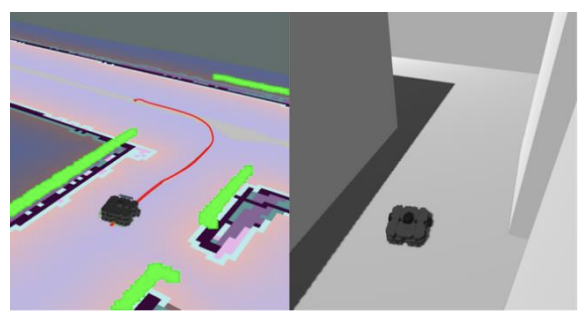
\includegraphics[height=40mm,width=80mm]{./figs/map_base.png}
     \caption{Imitation learning of path-tracking}\label{fig:mapbase}
\end{figure}

\section{カメラ画像を入力とする経路追従}
この手法では,カメラ画像とシナリオに基づいて,目的地まで自律移動する.
ここではまず初めに全体の流れについて述べた後,
それぞれの詳細を述べる.
手法のシステム概要をFig.\ref{fig:system}に示す.
\begin{figure}[h!]
    \centering
     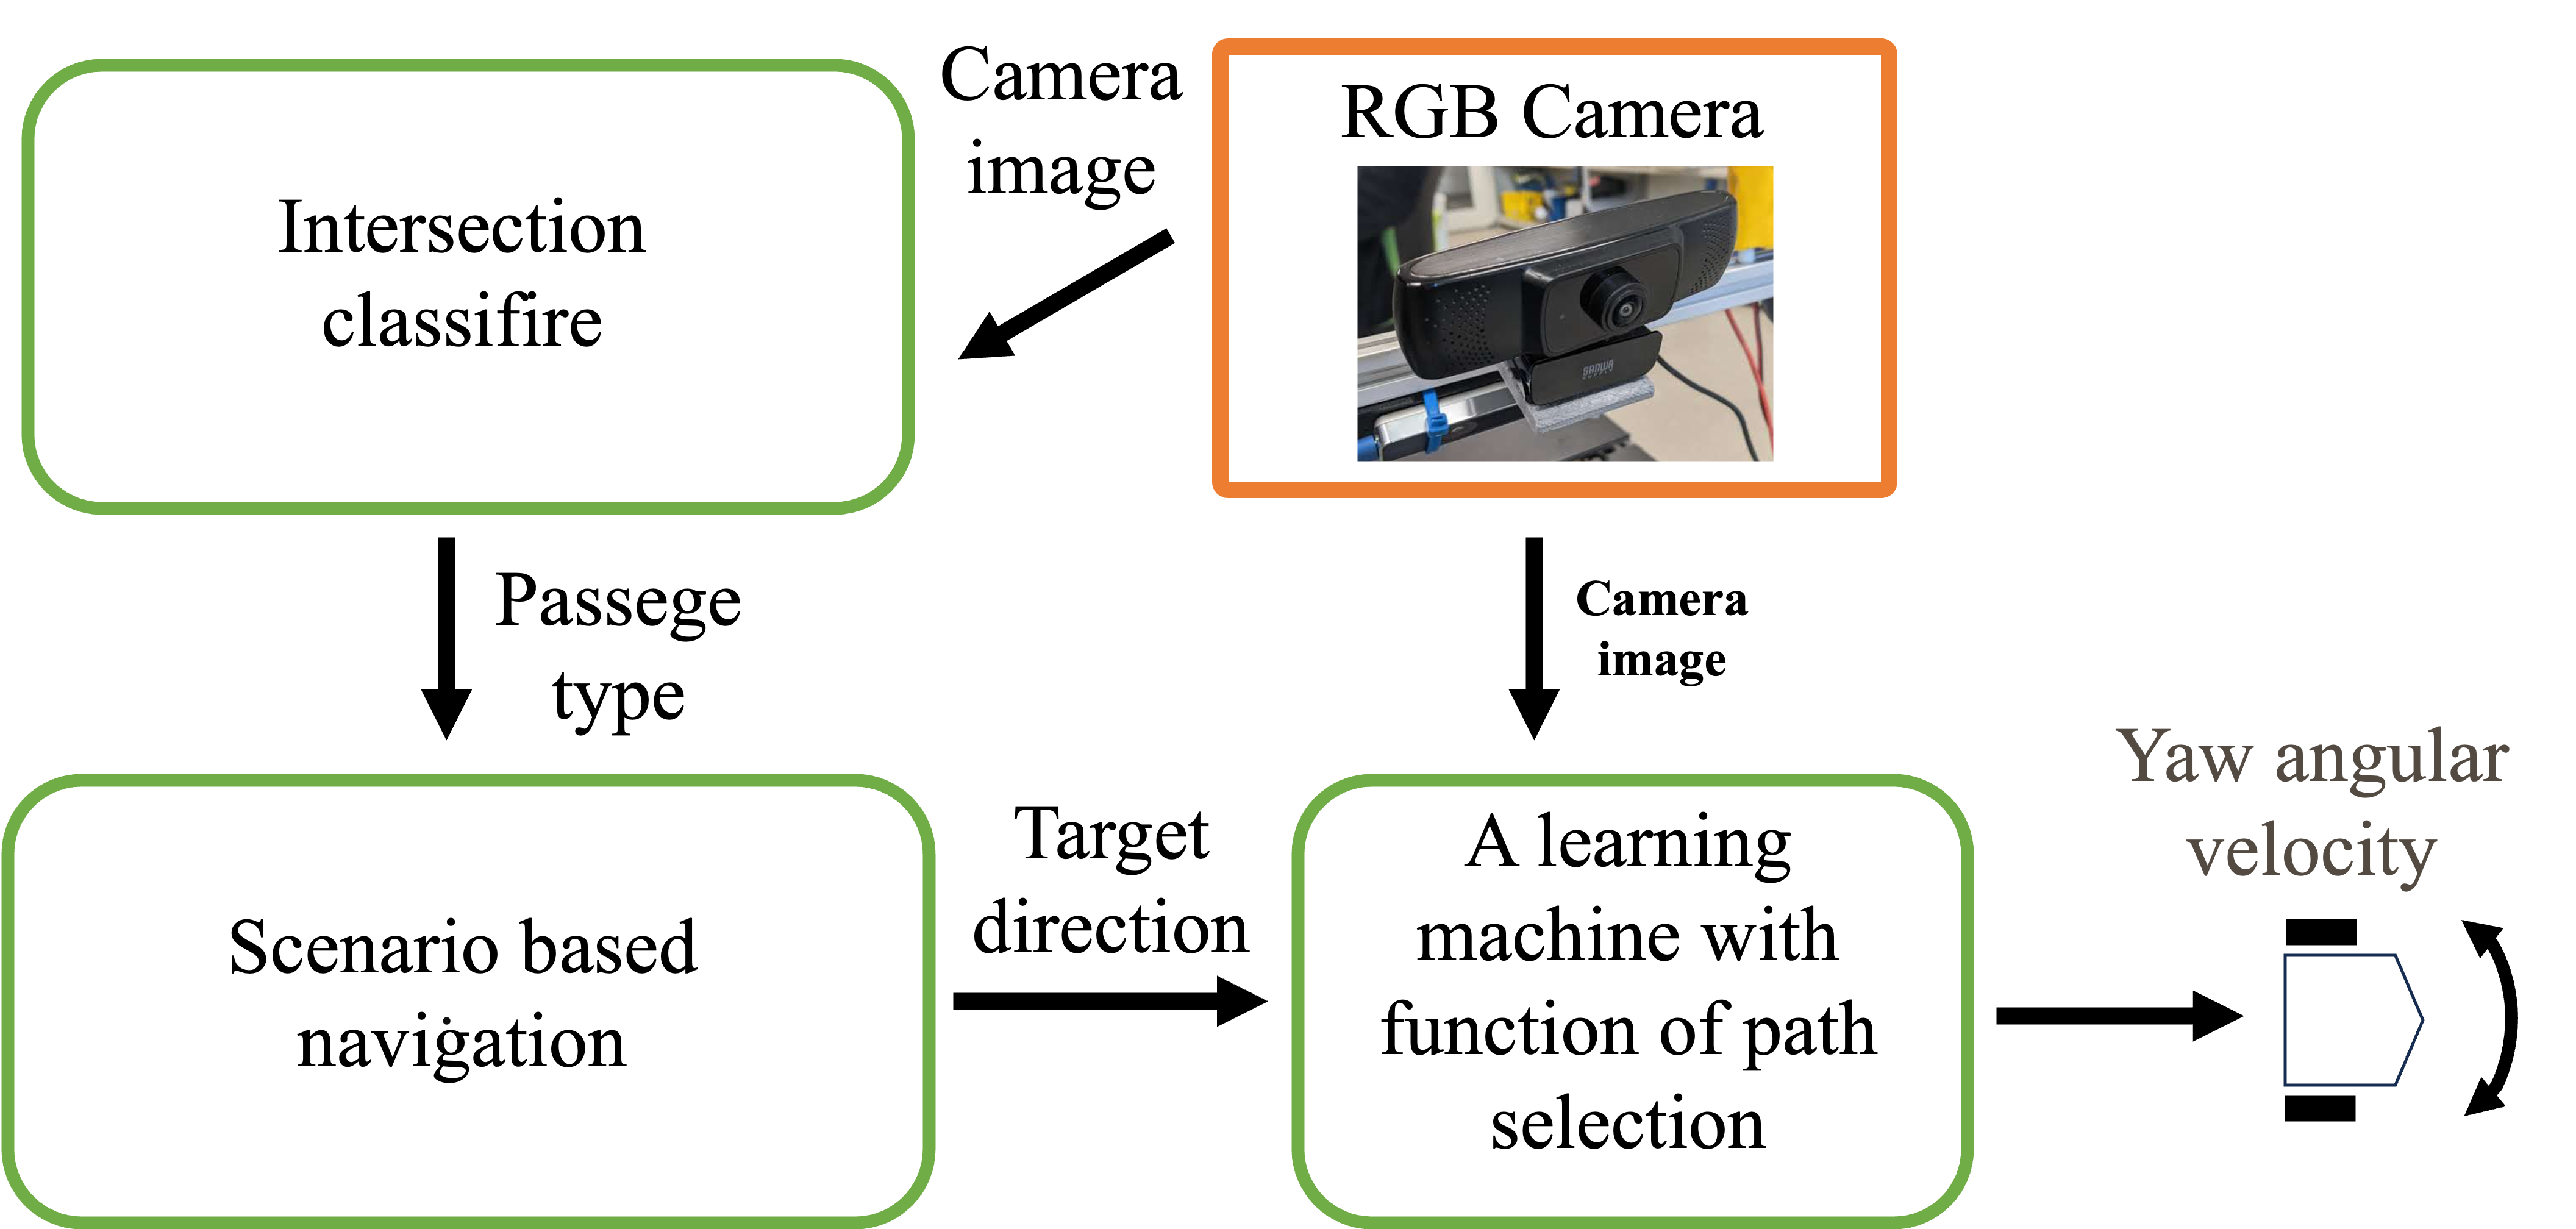
\includegraphics[height=40mm,width=70mm]{./figs/system_gai.png}
     \caption{Methods system overview}\label{fig:system}
\end{figure}
\par
システムは,RGBカメラをセンサ入力とし,\\
1)カメラ画像を入力とする通路分類器\\
2)シナリオに基づいたナビゲーション\\
3)経路選択機能を持つ学習器\\
の3つのモジュールで構成されている.

2)に対してシナリオを入力し,経路の設定を行う.
カメラから得た画像データを1)の通路分類器に入力する.
2)は通路分類器が出力する通路の特徴を基に,目標方向を生成する.
3)は2)から生成された目標方向とカメラから得た画像データを基に,
ヨー方向の角速度を出力する.
ロボットは3)から出力された角速度を基に経路を追従する.


\subsection{経路選択機能を持つ学習器}
学習器のシステムをFig.\ref{fig:learning}に示す.
学習時は,2D-LiDARやオドメトリ,占有格子地図に基づく,
地図ベースの制御器(ROS Navigation Stack\cite{ros-navigation})によって,設定した経路を走行する.
その際,入力をカメラ画像,目標方向,
地図ベースの制御器が出力するヨー方向の角速度を目標出力として,データセットに加える.
さらに,設定したバッチサイズ分の教師データをデータセットから抽出し,
オンラインで模倣学習を行う.この1連の流れを1ステップとする.
データセットの収集には,
\cite{fujiwara2023}
% [藤原]
で提案された,データセットの不均衡の改善,
学習時における積極的な蛇行といった最も成功率の高い手法を用いる.\par
学習後,訓練した学習器に対してカメラ画像と目標方向を入力し,
出力されるヨー方向の角速度,設定した並進速度によりロボットを制御する.
本稿では,並進速度を0.2m/sに設定する.
\cite{haruyama2022}\cite{fujiwara2023}では
% [春山][藤原]
学習後も,
地図ベースの制御器から生成される目標方向を用いていた.
本稿では,次の小節で述べるシナリオに基づくナビゲーションから生成する.
なお学習器のネットワークは
\cite{haruyama2022}\cite{fujiwara2023}
% [春山][藤原]
と同様の構成を用いる.
\begin{figure}[h!]
    \centering
     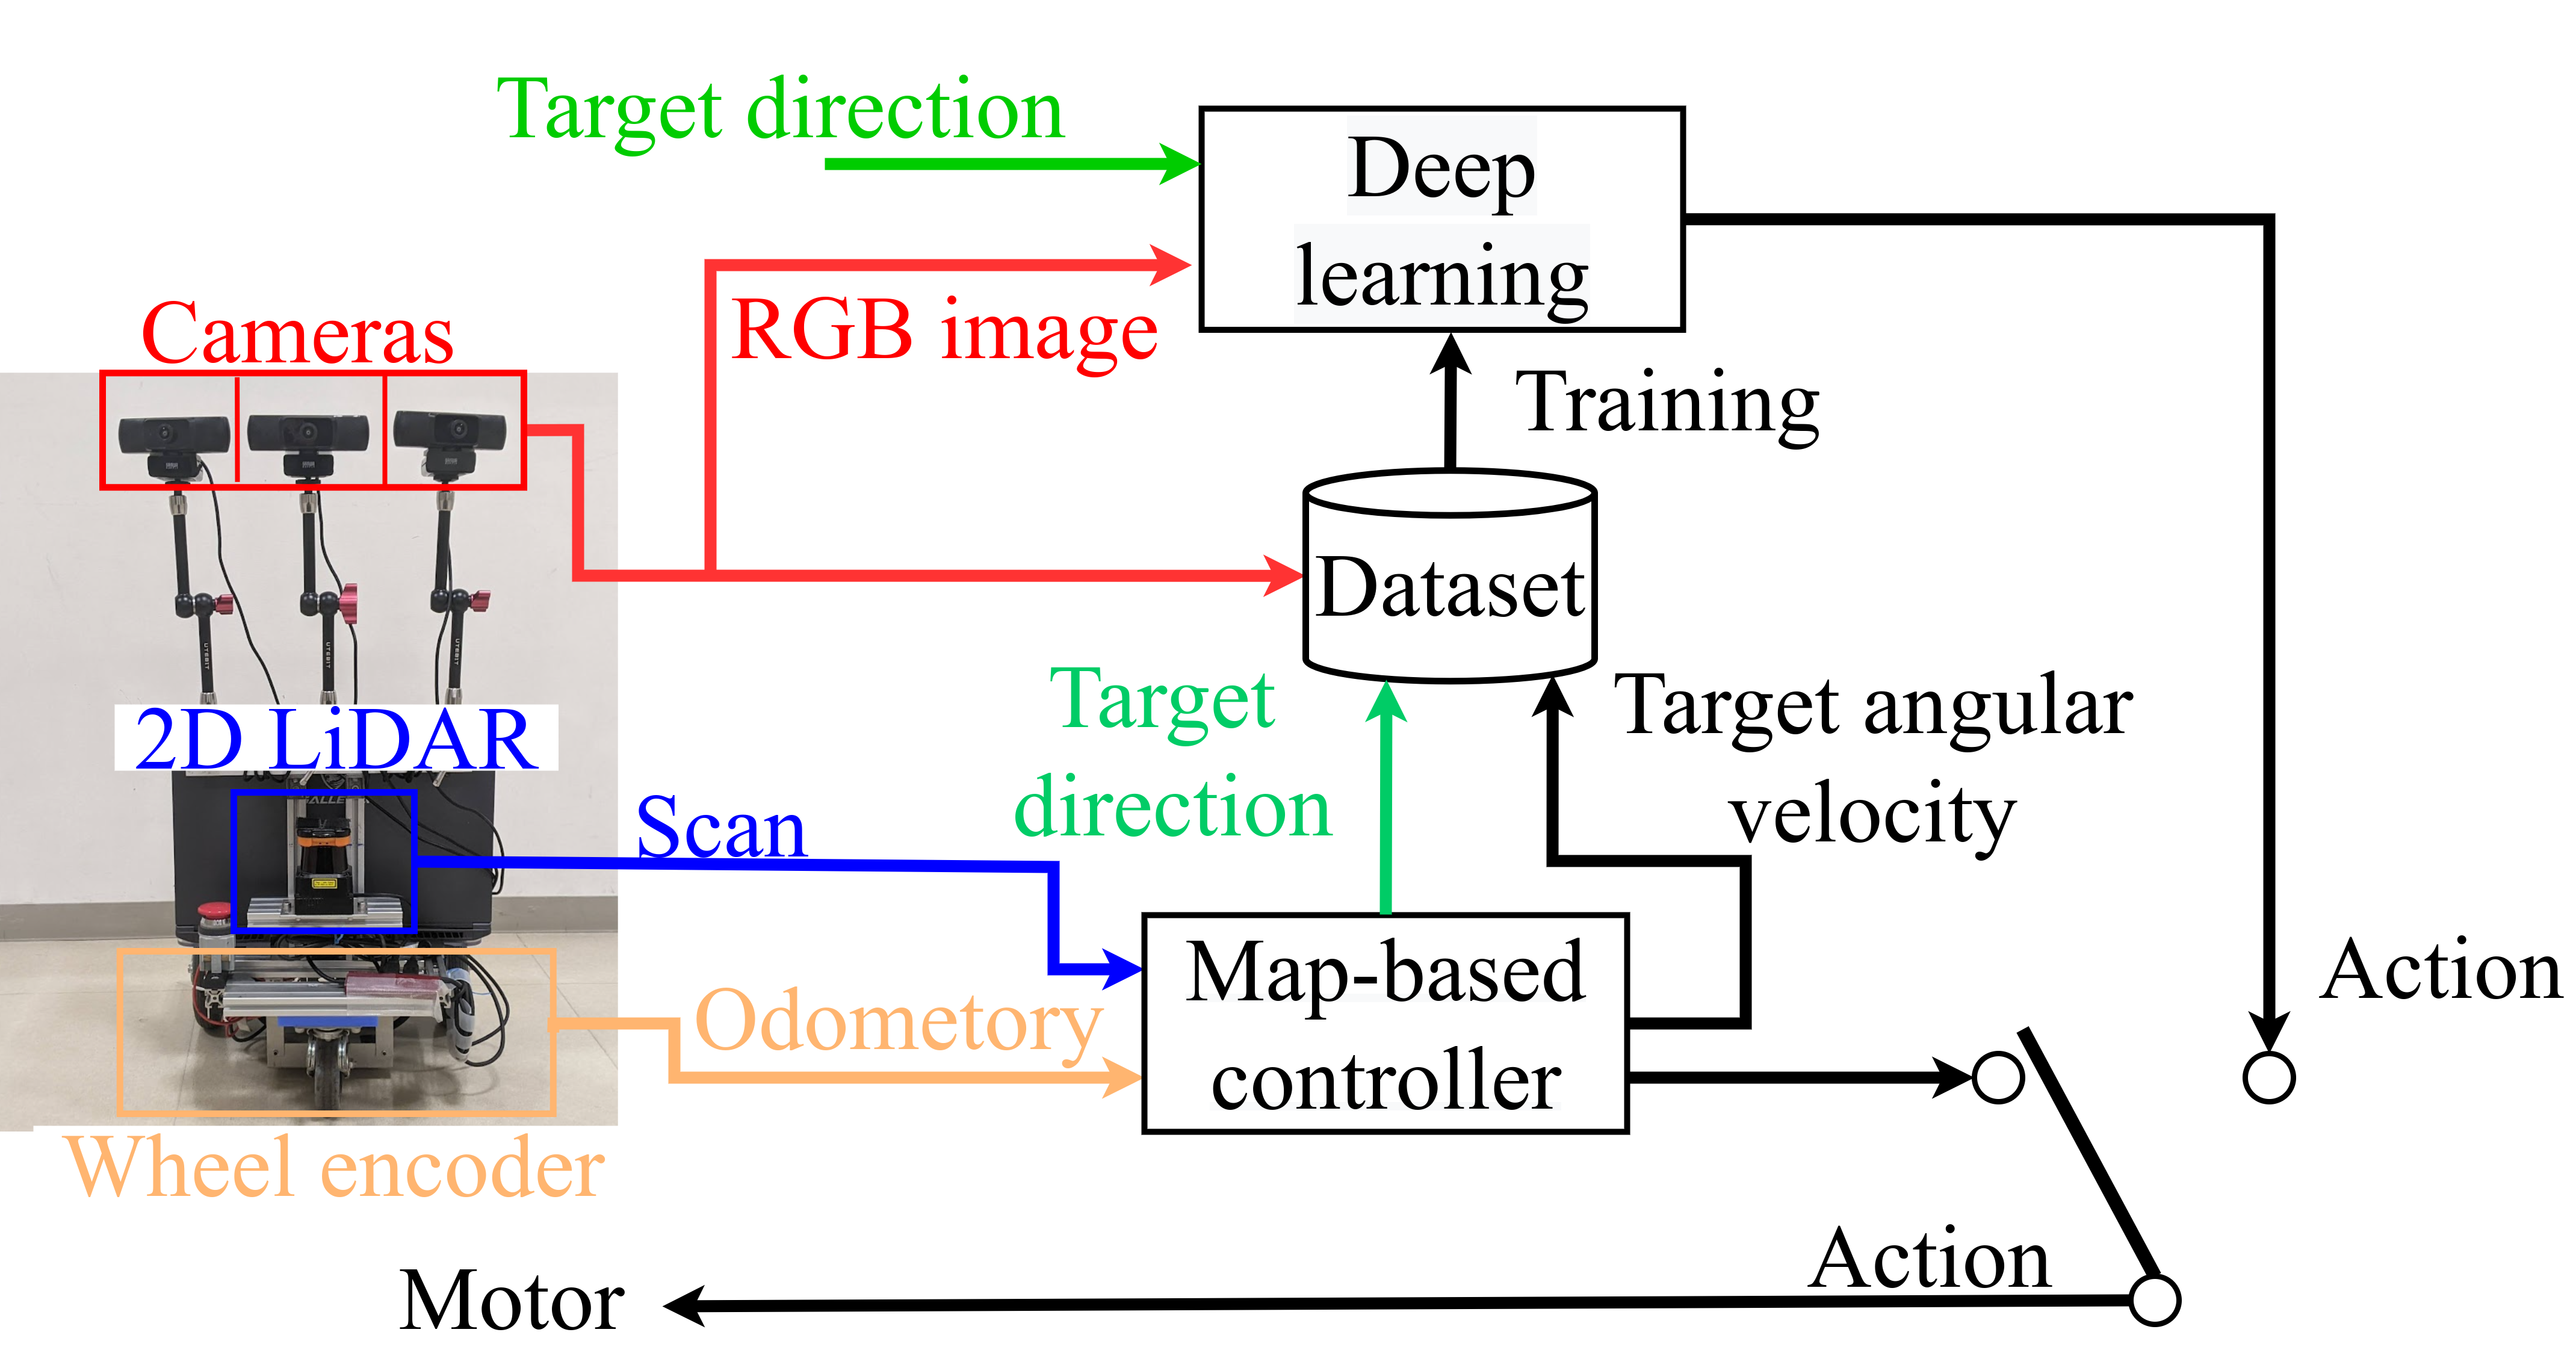
\includegraphics[height=45mm,width=80mm]{./figs/learning_gamma.png}
     \caption{Imitation learning system with target direction}\label{fig:learning}
\end{figure}
\subsection{シナリオに基づいたナビゲーション}
目的地までの経路の設定および,目標方向の生成を行う
シナリオに基づいたナビゲーションについて述べる.
このナビゲーションは\cite{shimada2020}
% [島田ら]
で提案された人の道案内情報を収集・分析し,
そのデータを基にトポロジカルマップの形式とシナリオ(経路の表現)を用いて
ロボットをナビゲーションする手法をベースに構成する.
% ~にトポロジカルマップとシナリオの例を示す.
\par
目標方向は\cite{shimada2020}
% [島田]
で開発された
1)シナリオからロボットの制御用の手順を生成する機能を拡張して生成する.
「3つ目の三叉路まで直進.右折.突き当たりまで直進.停止」
というシナリオの例を基に1)の機能と目標方向の生成について述べる.
この機能では,シナリオを句点ごとに分解後,
「条件」と「行動」を示す言葉を抽出し,以下の項目に分けて登録する.\\
1)通路の特徴\\
2)順番\\
3)方向\\
4)行動\\
シナリオの例は句点ごとに
3つ目の三叉路まで直進/ 
右折/ 
突き当たりまで直進/ 
停止/ 
と区切られる.
1つ目の区切りでは
1)通路の特徴:三叉路\\
2)順番:3\\
4)行動:直進\\
2つ目の区切りでは\\
4)行動:右折\\
が登録される.
この一連の作業を末尾の区切りである「停止」が登録されるまで行う.
ここで登録される「行動」をTable \ref{tab:target}に示すワンホットベクトルで表現し,
目標方向として,前述の学習器へ与える.

\begin{table}[]
    \centering
    \caption{Target direction and data for imitation learning}\label{tab:target}
    \begin{tabular}{|c|c|}
    \hline
    Target direction & Data        \\
    \hline
    Go straight   & {[}1,0,0{]} \\
    Turn left   & {[}0,1,0{]} \\
    Turn right   & {[}0,0,1{]} \\
    stop   & {[}0,0,0{]}\\
    \hline
    \end{tabular}
    \end{table}

\par
島田らは1)の機能の他に2)通路の特徴を検出する機能
3)経路に沿って通路を走行する2つの機能を開発している.
しかし,\cite{shimada2020}\cite{hara2022}
% [島田][原]
の手法では2)と3)にLiDARや全天球カメラのセンサ入力を
必要としている.
そのため,本稿では.
2)の通路の特徴検出を,次の小節で述べるカメラ画像による手法,
3)に関しては前述した経路選択機能をもつ学習器へ変更している.

\subsection{カメラ画像を用いた通路分類}
カメラ画像と機械学習を用いた通路分類器について述べる.
通路分類器の概要をFig.\ref{fig:lrcn}に示す.通路分類器は
シーケンスの画像データを入力とし,通路の特徴の分類を出力する.
通路の特徴の分類は\cite{shimada2020}に倣い,Fig.\ref{fig:intersection}に示した8つとする.
\begin{figure}[h!]
    \centering
     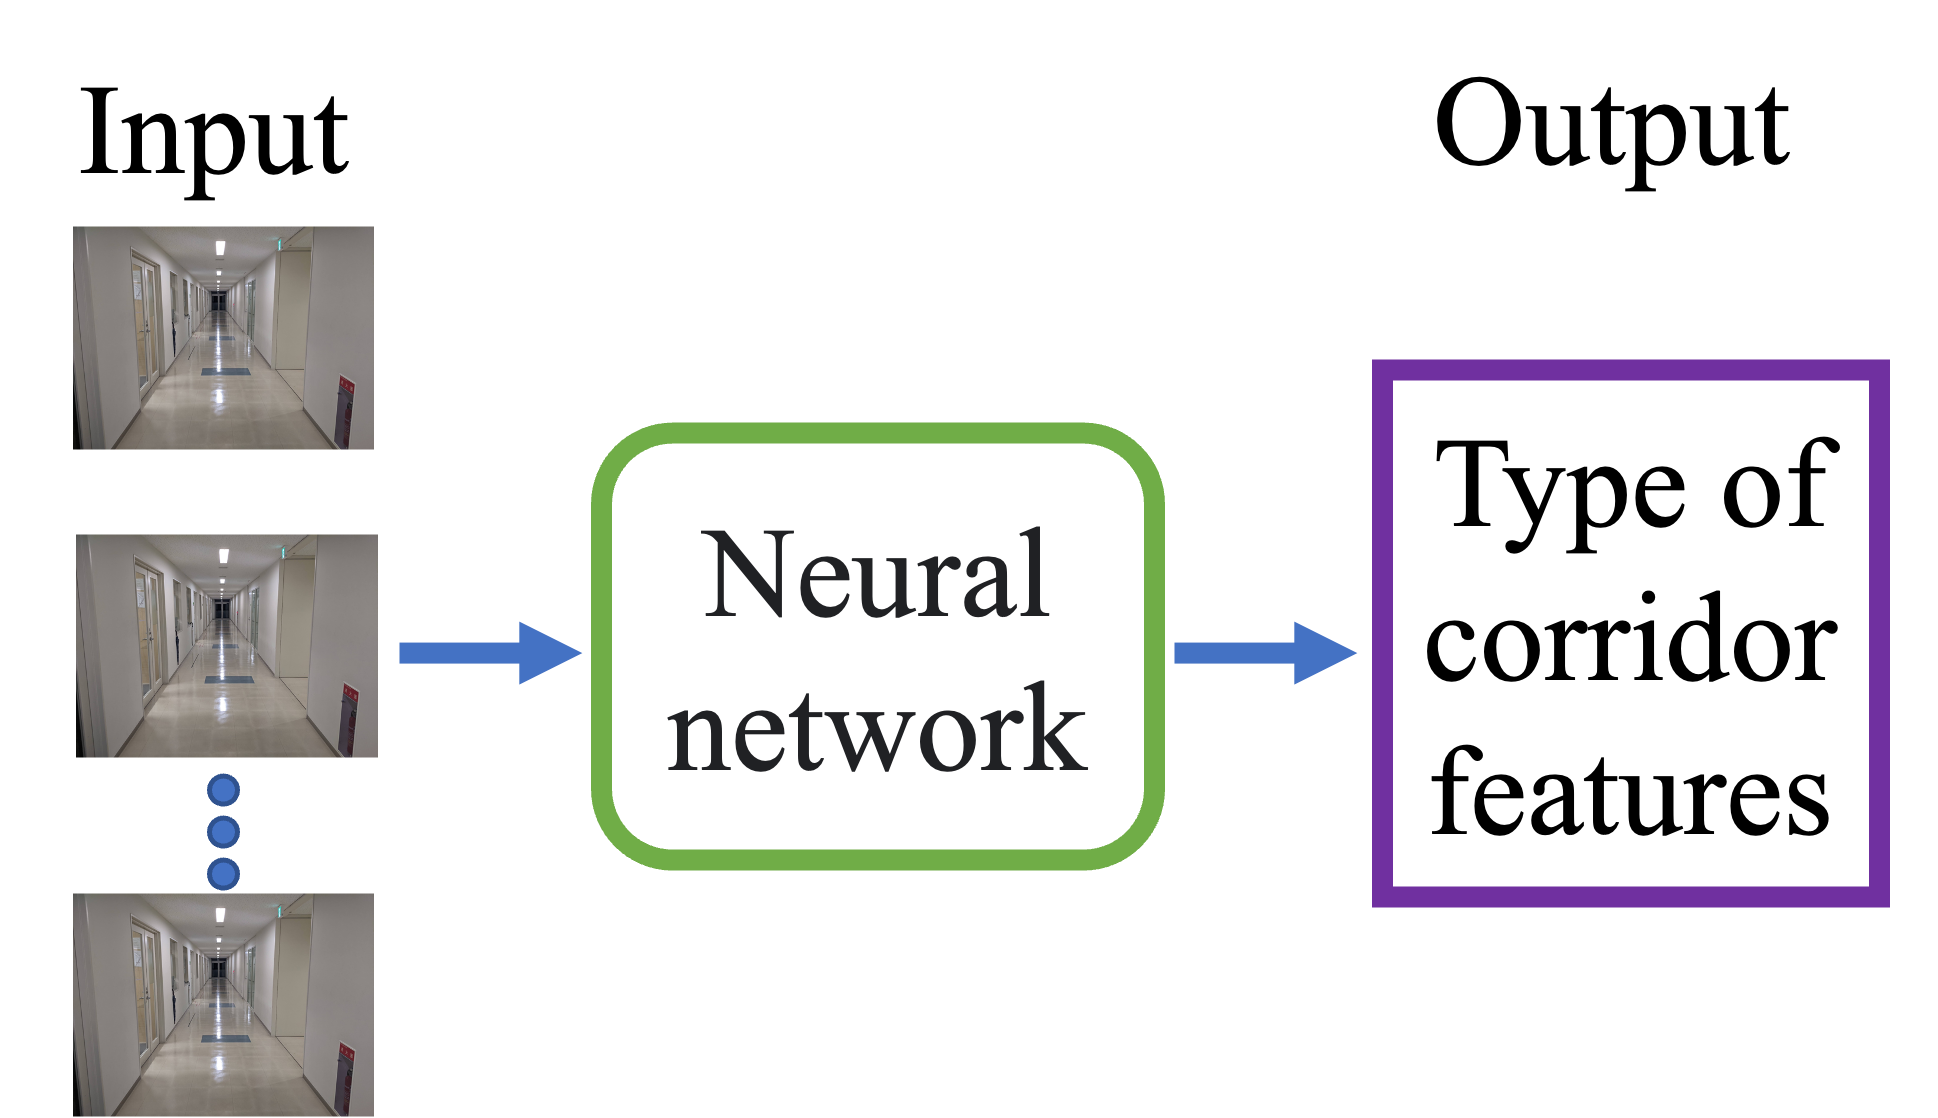
\includegraphics[height=40mm,width=80mm]{./figs/LRCN_gai.png}
     \caption{Types of corridor features classifier overview}\label{fig:lrcn}
\end{figure}
\begin{figure}[h!]
    \centering
     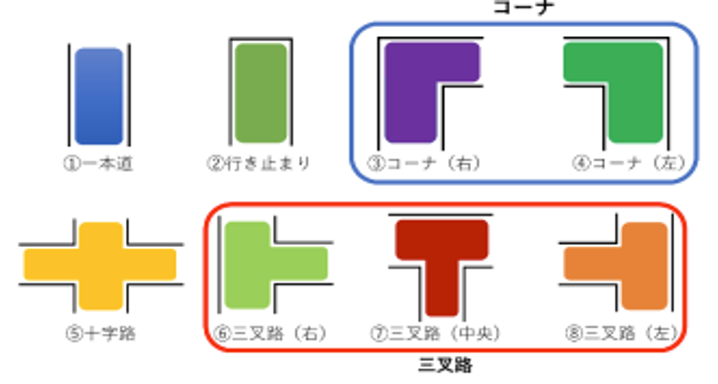
\includegraphics[height=40mm,width=80mm]{./figs/intersection.png}
     \caption{Types of corridor features\cite{shimada2020}}\label{fig:intersection}
\end{figure}
\par
通路分類器のネットワークアーキテクチャは
Dhaivatらが提案するCNNとLSTMを組み合わせたLRCN\cite{lrcn}を参考として構築した.
なお本稿では,CNNアーキテクチャをMobileNetV3-Large\cite{v3},
シーケンスデータのフレーム数は16 入力画像サイズを64x48 出力8へ変更している.
\par
学習するデータセット内で,各クラスのデータ数が大きく異なる不均衡データは,
分類に大きな影響を与える
\cite{hukin}
とされている.
そのため,本稿では学習する際に,データセット内のクラス間のデータ数によって
重み付けを行うコストアプローチ\cite{cost}を導入している.

\section{実験}
経路選択機能をもつ学習器に対して,シナリオに基づいたナビゲーションから
生成した目標方向を与える.
これにより,カメラ画像に基づいて指示された経路に従い,目的地へ到達可能であるか
検証する実験を行う.

\subsection{実験装置}
実験にはFig.\ref{fig:gamma}で示す本学で開発しているORNE-gammaをベースに,
カメラを3つ搭載したロボットを使用する.
\begin{figure}[htbp]
    \centering
     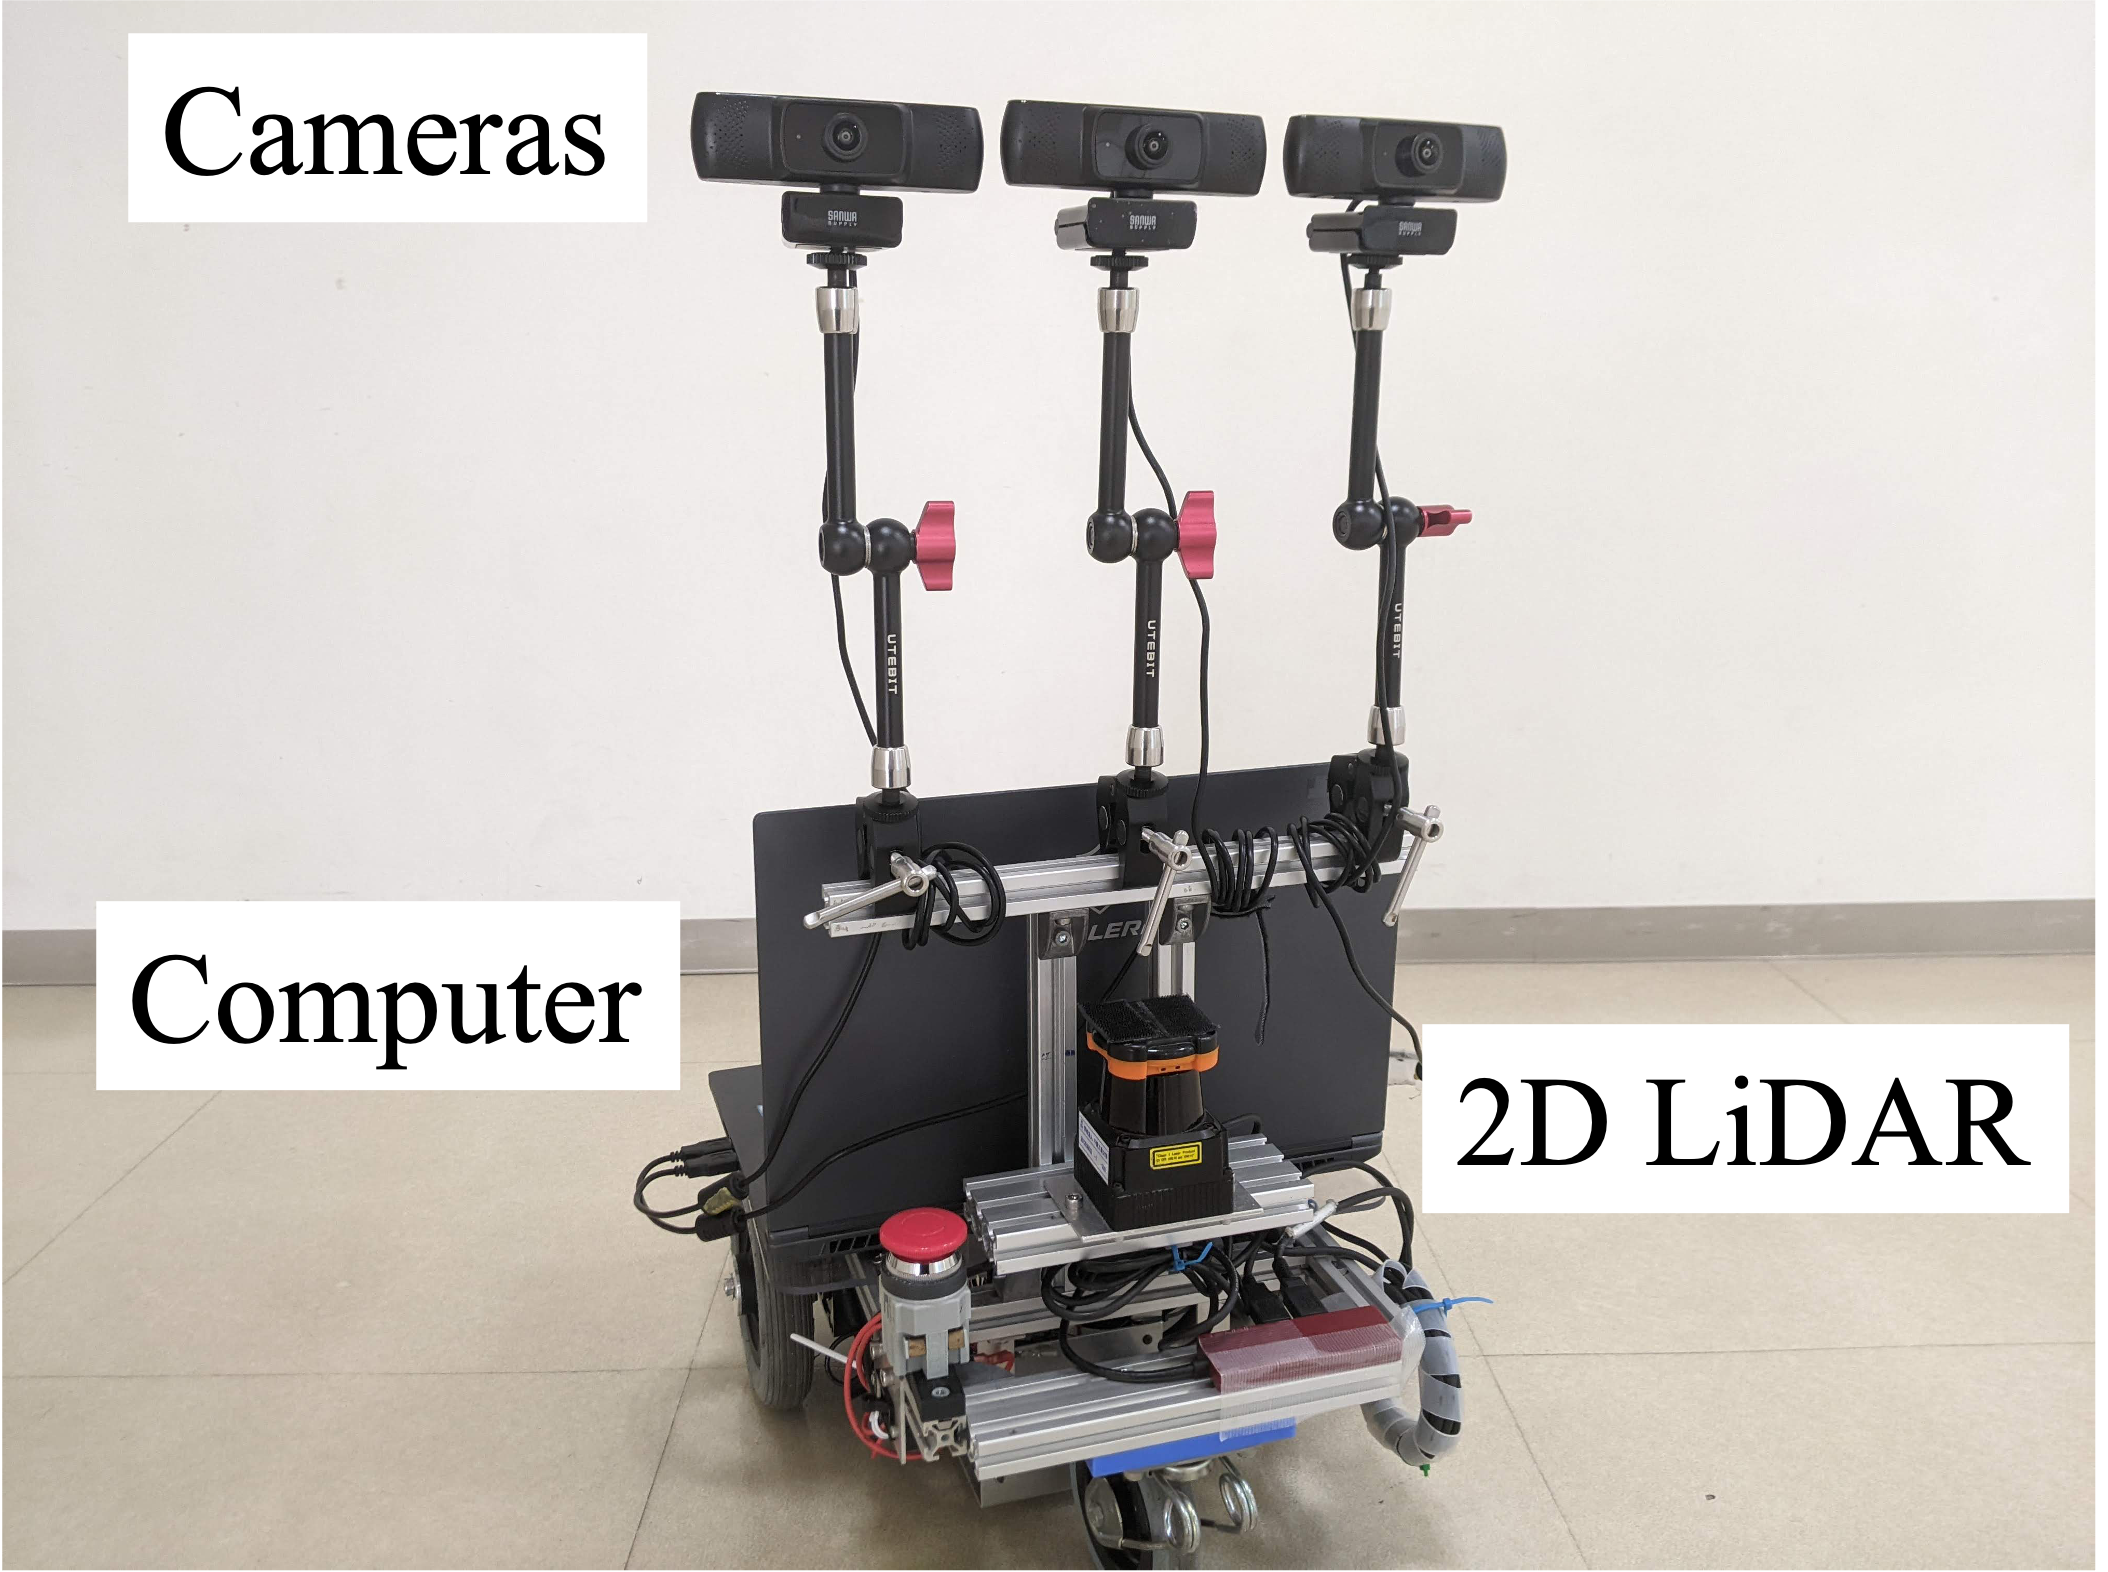
\includegraphics[height=50mm]{./figs/gamma_sensor.png}
     \caption{Experimental setup}\label{fig:gamma}
\end{figure}
\subsection{実験方法}
実験環境としてFig.\ref{fig:cit3f}で示した千葉工業大学津田沼キャンパス2号館3階の廊下を用いる.
% [藤原]と比較すると,突き当りが追加され,
% CとDが2つのこと行動を取ることが可能な分岐路へ変化している.
% 経路[藤原]で用いたa~fに図=で示したc~を追加した,a~nの順で走行する
[藤原]と比較すると,突き当り,2つのこと行動がとれる分岐路C,Dが追加されている.
経路は[藤原]で用いたaからfの経路へFig.\ref{fig:newroute}で示したgからnを加えた,
aからnを順番に走行する.\par
まず初めに通路分類器の訓練を行う.
前述の経路を地図ベースの制御器の出力を用いて,3周し,データセットを収集する.
その際,データセットへのデータの追加は0.125秒周期で行う.
1,2周目のデータを訓練データとし,3周目のデータをテストデータとする.
それぞれのデータセットを構成するシーケンス画像の個数は
訓練データは5781個,テストデータは2902個である.
訓練はバッチサイズは32として,30epoch行った.
訓練の結果,テストデータに対するAccuracyは0.98となった.\par
次に経路選択機能を持つ学習器の訓練を行う.
通路分類器の訓練と同様の経路を,オンラインで模倣学習しながら1周走行する.
その際のステップ数は〜である.
データセットへのデータの追加は0.25秒周期で行う.\par
実験では島田らが用いた50例のシナリオの中から,
Fig.\ref{fig:cit3f}に示したエリアを対象とした7例を抽出して用いる.
その際,1.地図ベースの制御器で通行が困難な場所が含まれるもの.
2.その場で「右を向く」といった学習器の出力を用いた走行では達成が困難なもの
を除外している.\par
抽出した7例のうちの1例のシナリオ,
また訓練した通路分類器と経路選択機能を持つ学習器をシステムにセットする.
その後,シナリオのスタート地点へシナリオに基づいた向きでロボットを配置し,
実験を開始する.
なお,経路から外れるといった要因で走行が困難になった場合でも即時失敗とせず,
失敗箇所を記録しながら,人間が介入し,実験を継続する.
Fig.\ref{fig:scenario24}に実験で用いたシナリオの1例を示す.
今回は,実験環境を2号館3階の一部のエリアに限定しているが,
今後はフロア全体へ拡張する予定である.
\begin{figure}[htbp]
    \centering
     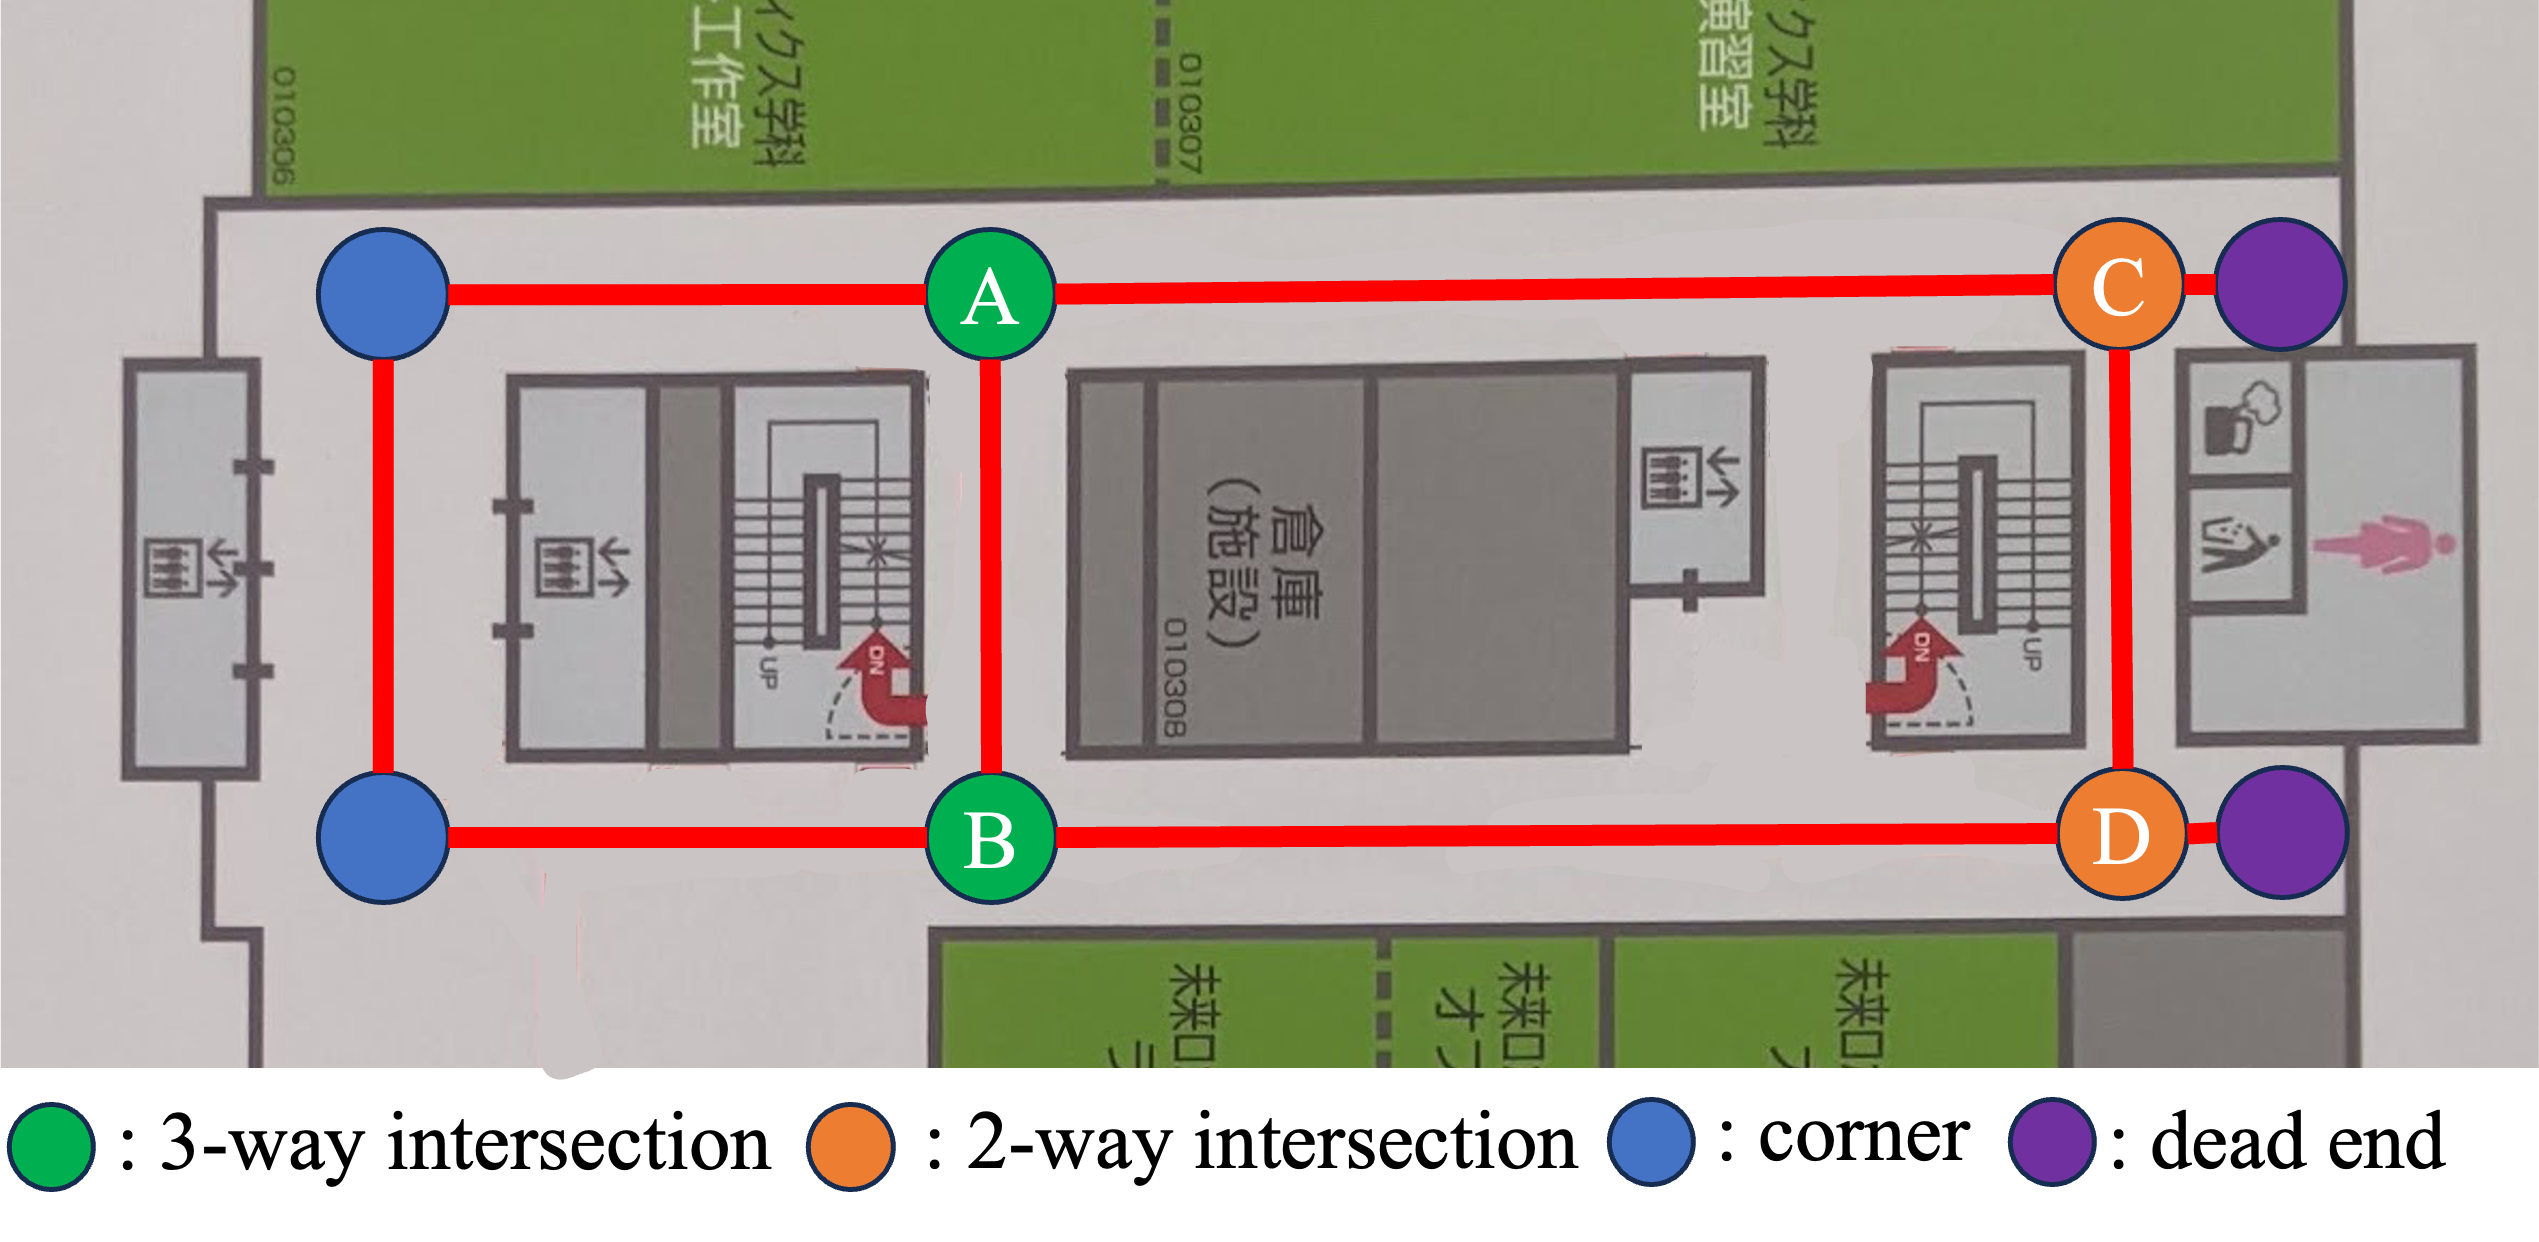
\includegraphics[height=40mm,width=80mm]{./figs/keiro.png}
     \caption{Experimental environment}\label{fig:cit3f}
\end{figure}
\begin{figure}[htbp]
    \centering
     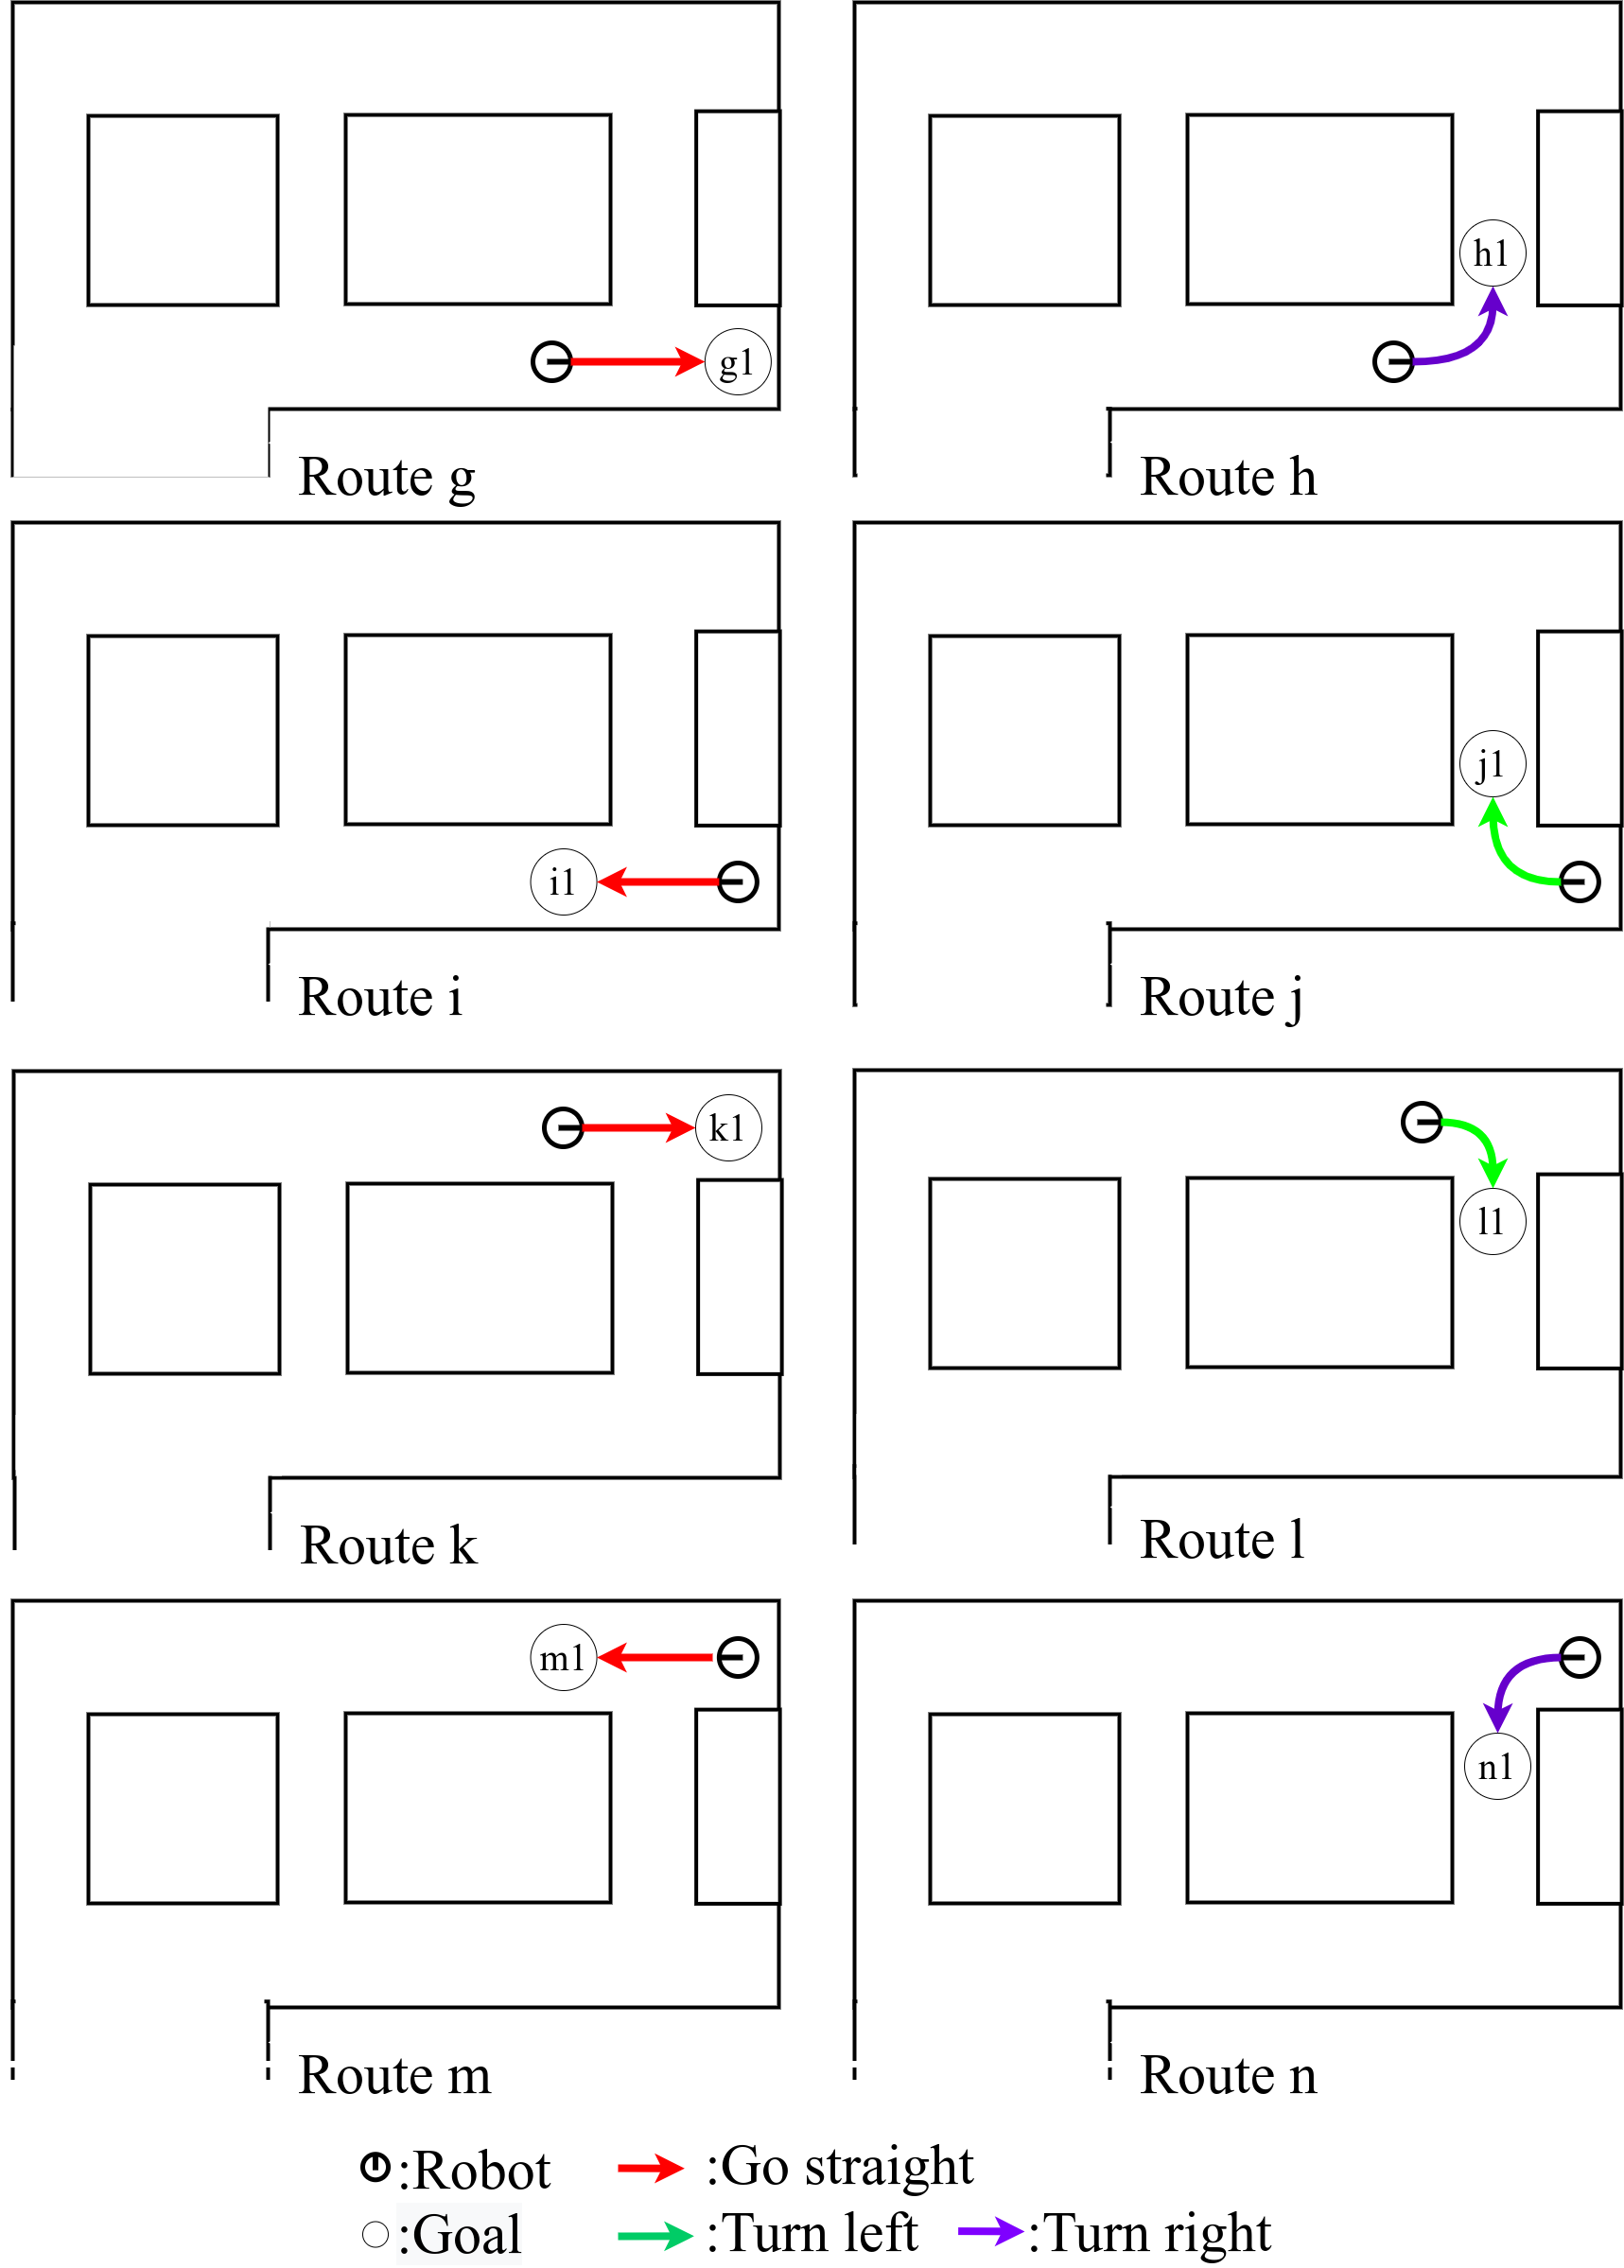
\includegraphics[height=100mm,width=80mm]{./figs/newroute.png}
     \caption{Route for the added experiment}\label{fig:newroute}
\end{figure}

\begin{figure}[h!]
    \centering
     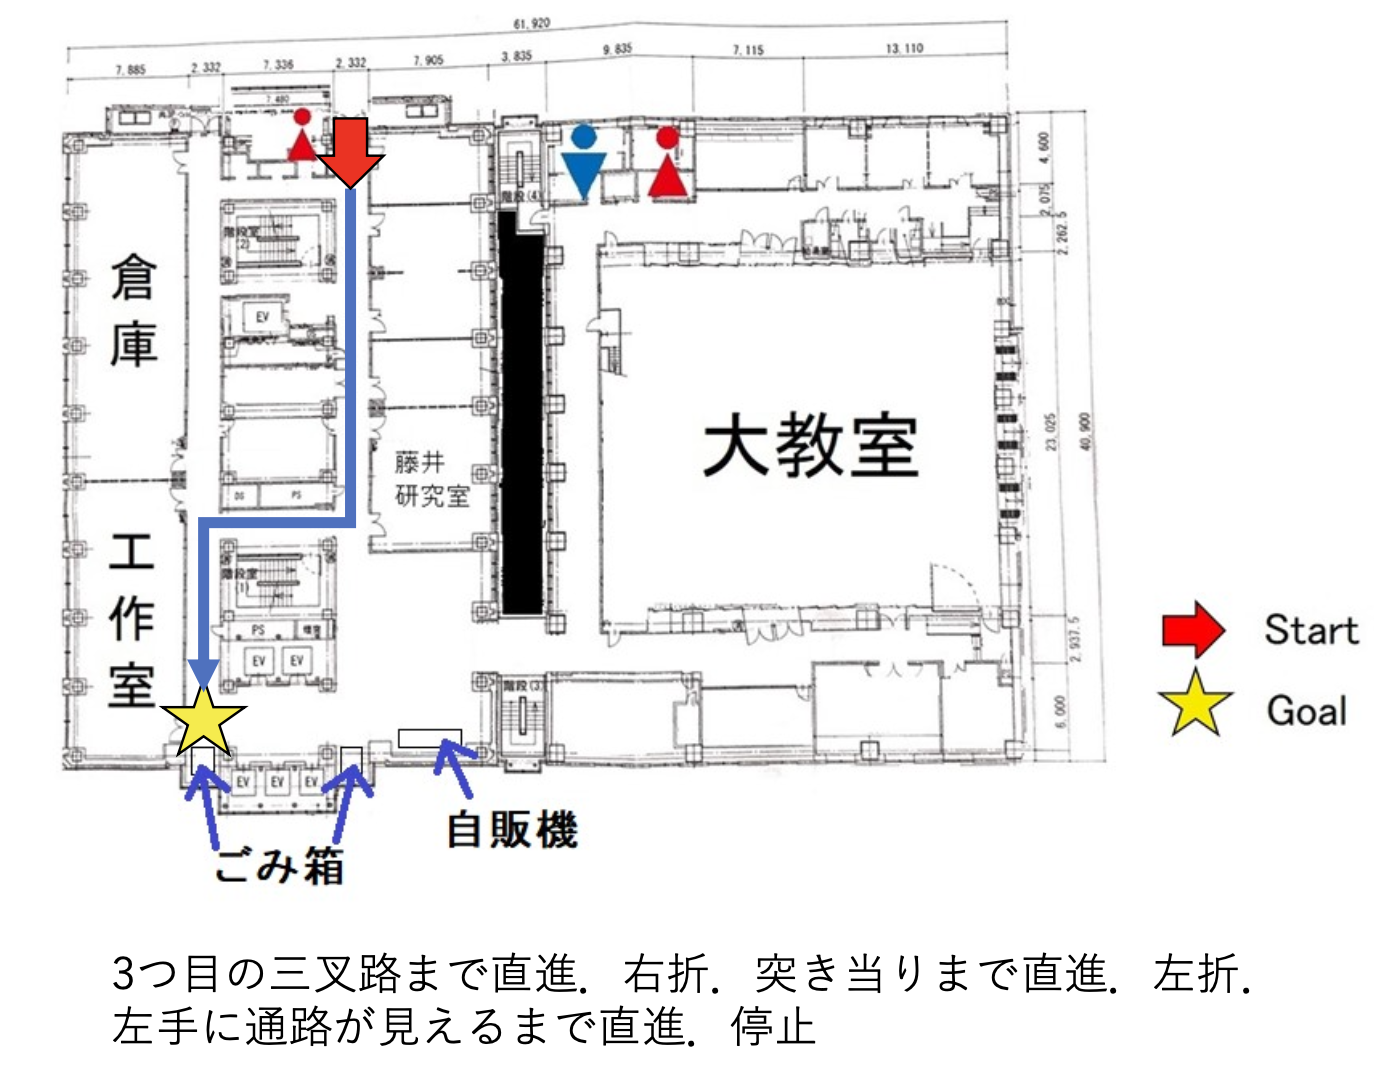
\includegraphics[height=50mm]{./figs/scenario24.png}
     \caption{Example of the scenario}\label{fig:scenario24}
\end{figure}
% \begin{figure}[htbp]
% \begin{center}
% 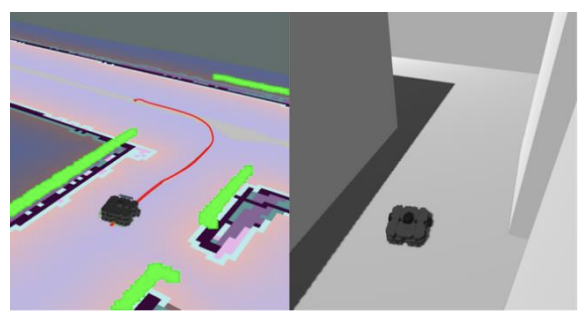
\includegraphics[height=50mm width=70mm]{./figs/map_base.png}
% \caption{ガザニア}
% \end{center}
% \end{figure}

\subsection{実験結果}
実験結果をTable \ref{tab:result}に示す.
表はそれぞれ実験に用いたシナリオの番号,学習器の出力が要因による介入の回数,
通路分類の間違いを原因とする介入の回数である.
結果として,抽出した7例のうち,7例すべての例で人間の介入なしで,
ロボットが指定された経路を追従して目的地へ到達した.
以上の結果から,経路選択機能を持つ学習器に対して,
シナリオに基づくナビゲーションとカメラ画像による通路分類を追加したシステムが,
適切に動作することを確認した.
\begin{table}[]
    \centering
    \caption{The number of assistances in the experiment}\label{tab:result}
    % \begin{tabular}{ccclll}
        
    % \begin{tabularx}{\textwidth}{X|X|X}
    \begin{tabularx}{80mm}{|C|C|C|}
    \hline
    Scenario number used in the experiment & 
    Number of assistances for deviating from the path & 
    Number of assistances due to corridor classification failures \\
    \hline
    1       & 0         & 0             \\
    5       & 0         & 0             \\
    20      & 0         & 0             \\
    21      & 0         & 0             \\
    22      & 0         & 0             \\
    24      & 0         & 0             \\
    50      & 0         & 0             \\
    \hline
    % \end{tabular}
    \end{tabularx}
    \end{table}

\section{結言}
本稿では,経路選択機能を持つ学習器を用いた走行に対して,
カメラ画像からの目標方向の生成を目的として,シナリオを
用いたナビゲーションと通路分類器の
追加を行った.
実験から,シナリオとカメラ画像を用いて目標方向の生成を行い,
学習器がカメラ画像と生成された目標方向を用いて,
指定された経路に沿って目的地へ到達可能なことを確認した.
今後は,実験環境をより広い屋内,または屋外へと拡大する予定である.
% \printbibliography[title=参考文献]
% \printbibliography[title=参考文献]
\end{document}
